% Options for packages loaded elsewhere
\PassOptionsToPackage{unicode}{hyperref}
\PassOptionsToPackage{hyphens}{url}
%
\documentclass[
]{book}
\usepackage{lmodern}
\usepackage{amsmath}
\usepackage{ifxetex,ifluatex}
\ifnum 0\ifxetex 1\fi\ifluatex 1\fi=0 % if pdftex
  \usepackage[T1]{fontenc}
  \usepackage[utf8]{inputenc}
  \usepackage{textcomp} % provide euro and other symbols
  \usepackage{amssymb}
\else % if luatex or xetex
  \usepackage{unicode-math}
  \defaultfontfeatures{Scale=MatchLowercase}
  \defaultfontfeatures[\rmfamily]{Ligatures=TeX,Scale=1}
\fi
% Use upquote if available, for straight quotes in verbatim environments
\IfFileExists{upquote.sty}{\usepackage{upquote}}{}
\IfFileExists{microtype.sty}{% use microtype if available
  \usepackage[]{microtype}
  \UseMicrotypeSet[protrusion]{basicmath} % disable protrusion for tt fonts
}{}
\makeatletter
\@ifundefined{KOMAClassName}{% if non-KOMA class
  \IfFileExists{parskip.sty}{%
    \usepackage{parskip}
  }{% else
    \setlength{\parindent}{0pt}
    \setlength{\parskip}{6pt plus 2pt minus 1pt}}
}{% if KOMA class
  \KOMAoptions{parskip=half}}
\makeatother
\usepackage{xcolor}
\IfFileExists{xurl.sty}{\usepackage{xurl}}{} % add URL line breaks if available
\IfFileExists{bookmark.sty}{\usepackage{bookmark}}{\usepackage{hyperref}}
\hypersetup{
  pdftitle={Bygge statistisk modeller med kategoriske variabler (ANOVA, t-test)},
  pdfauthor={Christian Magelssen},
  hidelinks,
  pdfcreator={LaTeX via pandoc}}
\urlstyle{same} % disable monospaced font for URLs
\usepackage{color}
\usepackage{fancyvrb}
\newcommand{\VerbBar}{|}
\newcommand{\VERB}{\Verb[commandchars=\\\{\}]}
\DefineVerbatimEnvironment{Highlighting}{Verbatim}{commandchars=\\\{\}}
% Add ',fontsize=\small' for more characters per line
\usepackage{framed}
\definecolor{shadecolor}{RGB}{248,248,248}
\newenvironment{Shaded}{\begin{snugshade}}{\end{snugshade}}
\newcommand{\AlertTok}[1]{\textcolor[rgb]{0.94,0.16,0.16}{#1}}
\newcommand{\AnnotationTok}[1]{\textcolor[rgb]{0.56,0.35,0.01}{\textbf{\textit{#1}}}}
\newcommand{\AttributeTok}[1]{\textcolor[rgb]{0.77,0.63,0.00}{#1}}
\newcommand{\BaseNTok}[1]{\textcolor[rgb]{0.00,0.00,0.81}{#1}}
\newcommand{\BuiltInTok}[1]{#1}
\newcommand{\CharTok}[1]{\textcolor[rgb]{0.31,0.60,0.02}{#1}}
\newcommand{\CommentTok}[1]{\textcolor[rgb]{0.56,0.35,0.01}{\textit{#1}}}
\newcommand{\CommentVarTok}[1]{\textcolor[rgb]{0.56,0.35,0.01}{\textbf{\textit{#1}}}}
\newcommand{\ConstantTok}[1]{\textcolor[rgb]{0.00,0.00,0.00}{#1}}
\newcommand{\ControlFlowTok}[1]{\textcolor[rgb]{0.13,0.29,0.53}{\textbf{#1}}}
\newcommand{\DataTypeTok}[1]{\textcolor[rgb]{0.13,0.29,0.53}{#1}}
\newcommand{\DecValTok}[1]{\textcolor[rgb]{0.00,0.00,0.81}{#1}}
\newcommand{\DocumentationTok}[1]{\textcolor[rgb]{0.56,0.35,0.01}{\textbf{\textit{#1}}}}
\newcommand{\ErrorTok}[1]{\textcolor[rgb]{0.64,0.00,0.00}{\textbf{#1}}}
\newcommand{\ExtensionTok}[1]{#1}
\newcommand{\FloatTok}[1]{\textcolor[rgb]{0.00,0.00,0.81}{#1}}
\newcommand{\FunctionTok}[1]{\textcolor[rgb]{0.00,0.00,0.00}{#1}}
\newcommand{\ImportTok}[1]{#1}
\newcommand{\InformationTok}[1]{\textcolor[rgb]{0.56,0.35,0.01}{\textbf{\textit{#1}}}}
\newcommand{\KeywordTok}[1]{\textcolor[rgb]{0.13,0.29,0.53}{\textbf{#1}}}
\newcommand{\NormalTok}[1]{#1}
\newcommand{\OperatorTok}[1]{\textcolor[rgb]{0.81,0.36,0.00}{\textbf{#1}}}
\newcommand{\OtherTok}[1]{\textcolor[rgb]{0.56,0.35,0.01}{#1}}
\newcommand{\PreprocessorTok}[1]{\textcolor[rgb]{0.56,0.35,0.01}{\textit{#1}}}
\newcommand{\RegionMarkerTok}[1]{#1}
\newcommand{\SpecialCharTok}[1]{\textcolor[rgb]{0.00,0.00,0.00}{#1}}
\newcommand{\SpecialStringTok}[1]{\textcolor[rgb]{0.31,0.60,0.02}{#1}}
\newcommand{\StringTok}[1]{\textcolor[rgb]{0.31,0.60,0.02}{#1}}
\newcommand{\VariableTok}[1]{\textcolor[rgb]{0.00,0.00,0.00}{#1}}
\newcommand{\VerbatimStringTok}[1]{\textcolor[rgb]{0.31,0.60,0.02}{#1}}
\newcommand{\WarningTok}[1]{\textcolor[rgb]{0.56,0.35,0.01}{\textbf{\textit{#1}}}}
\usepackage{longtable,booktabs}
\usepackage{calc} % for calculating minipage widths
% Correct order of tables after \paragraph or \subparagraph
\usepackage{etoolbox}
\makeatletter
\patchcmd\longtable{\par}{\if@noskipsec\mbox{}\fi\par}{}{}
\makeatother
% Allow footnotes in longtable head/foot
\IfFileExists{footnotehyper.sty}{\usepackage{footnotehyper}}{\usepackage{footnote}}
\makesavenoteenv{longtable}
\usepackage{graphicx}
\makeatletter
\def\maxwidth{\ifdim\Gin@nat@width>\linewidth\linewidth\else\Gin@nat@width\fi}
\def\maxheight{\ifdim\Gin@nat@height>\textheight\textheight\else\Gin@nat@height\fi}
\makeatother
% Scale images if necessary, so that they will not overflow the page
% margins by default, and it is still possible to overwrite the defaults
% using explicit options in \includegraphics[width, height, ...]{}
\setkeys{Gin}{width=\maxwidth,height=\maxheight,keepaspectratio}
% Set default figure placement to htbp
\makeatletter
\def\fps@figure{htbp}
\makeatother
\setlength{\emergencystretch}{3em} % prevent overfull lines
\providecommand{\tightlist}{%
  \setlength{\itemsep}{0pt}\setlength{\parskip}{0pt}}
\setcounter{secnumdepth}{5}
\usepackage{booktabs}

\newenvironment{danger}
    {
    \hline\\
    }
    { 
    \\\\\hline
    }
    
\newenvironment{warning}
    {
    \hline\\
    }
    { 
    \\\\\hline
    }
    
\newenvironment{info}
    {
    \hline\\
    }
    { 
    \\\\\hline
    }
    
\newenvironment{try}
    {
    \hline\\
    }
    { 
    \\\\\hline
    }
\ifluatex
  \usepackage{selnolig}  % disable illegal ligatures
\fi
\usepackage[]{natbib}
\bibliographystyle{apalike}

\title{Bygge statistisk modeller med kategoriske variabler (ANOVA, t-test)}
\author{Christian Magelssen}
\date{2021-03-31}

\begin{document}
\maketitle

{
\setcounter{tocdepth}{1}
\tableofcontents
}
\hypertarget{intro}{%
\chapter{Introduksjon}\label{intro}}

I dette kapittelet skal vi lære å bygge statistiske modeller for å teste om \textbf{to eller flere grupper er forskjellige på en avhengig variabel som er kontinuerlig}.

En variabel kan sies å være \textbf{kontinuerlig} når vi kan bestemme hvor presist vi ønsker å måle den. For eksempel regnes tid som en kontuerlig variabel fordi det (i prinsippet) ikke finnes noen grenser hvor presist vi kan måle det; vi kan måle det i år, måneder, uker, dager, timer, minutter, sekunder, tideler, hundredeler eller tusendeler.

\textbf{Grupper} defineres i psykologifaget som en samling mennesker som deler bestemte karakterstikker. Det kan være spillere på et fotballag, individer på et treningssenter, eller menn og kvinner. Dette er også eksempler på naturlig inndelte grupper i samfunnet. Noen ganger kan det være interessant å se om disse gruppene er forskjellige. For eksempel kan det være interessant å se om individer som trener på treningssenter er sterkere enn de som ikke trener på treningssenter.

Andre ganger kan det være interessant å teste om to grupper, som var like før et eksperiment, har blitt forskjellige fordi vi har behandlet dem ulikt. Vi randomiserer individer i to ulike grupper, slik at vi sikrer at vi blander disse individene godt (f.eks kjønn, motivasjon, interesser). Hvis eksperimentet har blitt gjennomført godt at det ikke er noen andre forklaringer på at disse to gruppene har blitt forskjellige etter intervensjonsperioden, så kan vi trekke en slutning om disse to gruppene trolig ikke kommer fra samme populasjon lenger; eksperimentet har gjort at disse to gruppene trolig kommer fra to forskjellige populasjoner.

\hypertarget{datasett}{%
\chapter{Datasett}\label{datasett}}

\hypertarget{buxf8r-man-trene-med-ett-eller-flere-sett-i-styrketrening}{%
\section{Bør man trene med ett eller flere sett i styrketrening?}\label{buxf8r-man-trene-med-ett-eller-flere-sett-i-styrketrening}}

Et spørsmål mange treningsentusiaster lurer på er hvor mange serier som er best å gjennnomføre for å få maksimal treningseffekt i styrketrening. Noen mener at ett sett er tilstrekkelig, mens andre mener at et hardere treningstimuli er nødvendig og at to eller flere sett derfor er bedre. En forsker som var tidlig ute med å undersøke dette er deres egen Bent Rønnestad.

Eksperimentet ble gjennomført som et \textbf{between-subject design} med to grupper: en gruppe trente 1 sett på underkroppen og 3 sett på overkroppen; En annen gruppe trente 3 sett på underkroppen og 1 sett på overkroppen. Disse gruppene kalte han henholdsvis \textbf{1L-3U} og \textbf{3L-1U} (L=lower; U=Upper). De to gruppene trente 3 ganger i uken i totalt 11 uker. Forskerne ville så se hva som ga best fremgang på 1RM. Den avhengige variabelen ble derfor \%-fremgang på 1RM på underkroppsøvelser. De fant at 3L-1U hadde større fremgang enn 1L-3U fra pre til post (41 vs 21 \% endring). Denne forskjellen var signifikant ved en uavhengig t-test. Med andre ord kan det se ut til at det kan lønne seg å trene flere sett per styrketreningsøkt.

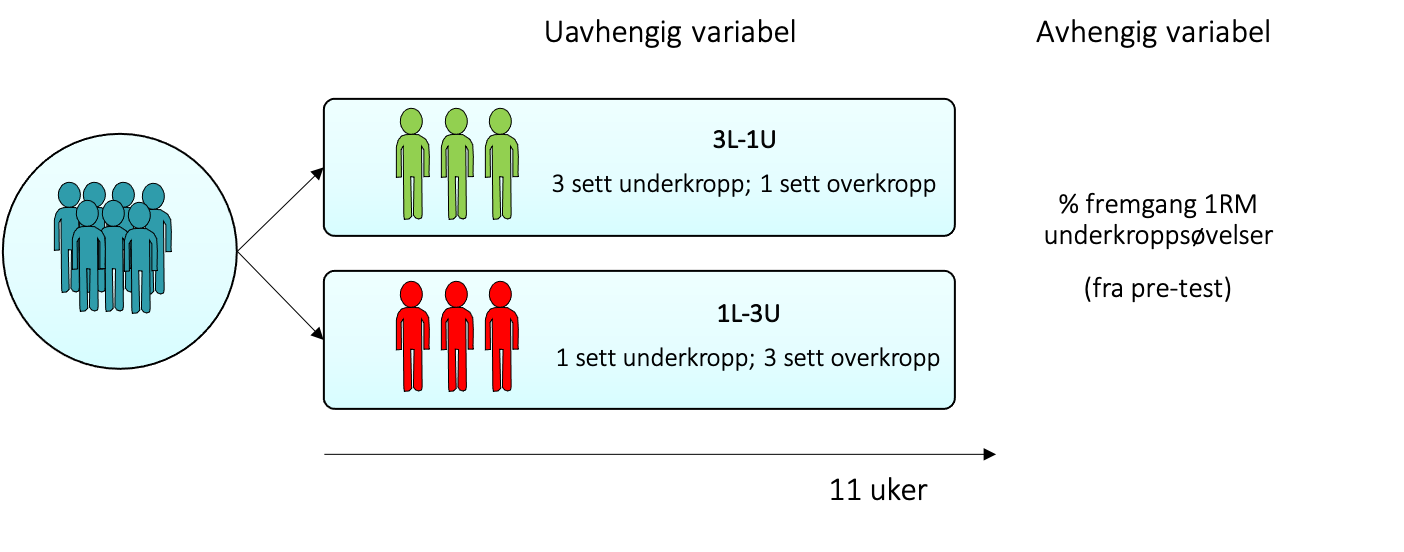
\includegraphics{design.png}
Vi har ikke tilgang til dette datasettet, men jeg har simulert dette datasettet i R basert på verdiene jeg fant i artikkelen. Datasettet blir tilnærmet likt, men siden det er en simulering blir det aldri helt identisk. Datasettet ser du i tabellen under.

\begin{table}

\caption{\label{tab:unnamed-chunk-3}Simulert datasett}
\centering
\begin{tabular}[t]{rlr}
\toprule
individ & gruppe & rm\\
\midrule
1 & tre.sett & 40.46704\\
2 & tre.sett & 49.07223\\
3 & tre.sett & 47.94131\\
4 & tre.sett & 44.51389\\
5 & tre.sett & 52.28750\\
\addlinespace
6 & tre.sett & 40.01750\\
7 & tre.sett & 49.48425\\
8 & tre.sett & 29.21048\\
9 & tre.sett & 40.59293\\
10 & tre.sett & 37.58676\\
\addlinespace
11 & tre.sett & 35.42651\\
12 & tre.sett & 42.49354\\
13 & ett.sett & 17.70576\\
14 & ett.sett & 17.07181\\
15 & ett.sett & 18.26811\\
\addlinespace
16 & ett.sett & 25.42594\\
17 & ett.sett & 32.70313\\
18 & ett.sett & 19.10226\\
19 & ett.sett & 22.23827\\
20 & ett.sett & 22.27148\\
\addlinespace
21 & ett.sett & 26.17889\\
22 & ett.sett & 20.34857\\
23 & ett.sett & 23.52773\\
24 & ett.sett & 17.95966\\
\bottomrule
\end{tabular}
\end{table}

Du kan få nøyaktig samme datsett ved å klippe ut og lime inn følgende kode i en skript-fil i R (husk å laste inn tidyverse-pakken, library(tidyverse) ). Du kan også laste ned datasettet som en .csv fil fra canvas.

\begin{Shaded}
\begin{Highlighting}[]
\FunctionTok{set.seed}\NormalTok{(}\DecValTok{2002}\NormalTok{) }\CommentTok{\#viktig å ha med denne for å få nøyaktig samme datasett}
\NormalTok{tre.sett }\OtherTok{\textless{}{-}} \FunctionTok{rnorm}\NormalTok{(}\AttributeTok{n =} \DecValTok{12}\NormalTok{, }\AttributeTok{mean =} \DecValTok{41}\NormalTok{, }\AttributeTok{sd =} \DecValTok{5}\NormalTok{) }\CommentTok{\#12 individer}
\NormalTok{ett.sett }\OtherTok{\textless{}{-}}\FunctionTok{rnorm}\NormalTok{(}\AttributeTok{n =} \DecValTok{12}\NormalTok{, }\AttributeTok{mean =} \DecValTok{21}\NormalTok{, }\AttributeTok{sd =} \DecValTok{5}\NormalTok{) }\CommentTok{\#12 individer}

\CommentTok{\#lager en tibble fra tidyverse{-}pakken. Må ha lastet inn tidyverse library(tidyverse) i scriptfilen}
\NormalTok{dat }\OtherTok{\textless{}{-}} \FunctionTok{tibble}\NormalTok{(}\AttributeTok{individ =} \FunctionTok{seq}\NormalTok{(}\DecValTok{1}\SpecialCharTok{:}\DecValTok{24}\NormalTok{),}
              \AttributeTok{gruppe =} \FunctionTok{rep}\NormalTok{(}\FunctionTok{c}\NormalTok{(}\StringTok{"tre.sett "}\NormalTok{, }\StringTok{"ett.sett"}\NormalTok{), }\FunctionTok{c}\NormalTok{(}\FunctionTok{length}\NormalTok{(tre.sett), }\FunctionTok{length}\NormalTok{(ett.sett))),}
              \AttributeTok{rm =} \FunctionTok{c}\NormalTok{(tre.sett , ett.sett))}
\end{Highlighting}
\end{Shaded}

Før du går videre er det greit at du gjør deg kjent med datasettet som vi har generert. Studer datasettet og svar på følgende spørsmål:

\begin{enumerate}
\def\labelenumi{\arabic{enumi}.}
\tightlist
\item
  Hvor mange kolonner er det i tabellen over?
\item
  Hvor mange deltakere var med i studien?
\item
  Hvilke to verdier kan variabelen gruppe? og
\end{enumerate}

\hypertarget{regne-gjennomsnitt-for-de-to-gruppene}{%
\section{Regne gjennomsnitt for de to gruppene}\label{regne-gjennomsnitt-for-de-to-gruppene}}

Bra! Det er alltid viktig å bli kjent med sitt eget datasett, men nå som du har det kan vi gå videre. Vi er interessert i om det er forskjeller mellom de to gruppene (``tre.sett'' vs.~ett.sett) på \% fremgang fra pre- til post-test. Så kanskje vi kan starte med å se om det er forskjeller i gjennomsnitt mellom to gruppene? Dette kan enkelt gjøres i R, Jamovi eller excel. Her er en kode for å gjøre dette i R:

\begin{Shaded}
\begin{Highlighting}[]
\CommentTok{\#jeg lager et oobjekt som heter mean\_rm }
\NormalTok{mean\_rm }\OtherTok{\textless{}{-}}\NormalTok{ dat }\SpecialCharTok{\%\textgreater{}\%}
  \CommentTok{\#Jeg grupperer etter gruppe, slik at jeg får et mean for hver gruppe istf. for å få mean for alle individene}
  \CommentTok{\#group\_by er en funksjon for dette}
  \FunctionTok{group\_by}\NormalTok{(gruppe) }\SpecialCharTok{\%\textgreater{}\%}
  \CommentTok{\#deretter bruker jeg summarise funksjonen for å regne gjennomsnitt}
  \FunctionTok{summarise}\NormalTok{(}\AttributeTok{mean.fremgang.1RM =} \FunctionTok{mean}\NormalTok{(rm))}
\end{Highlighting}
\end{Shaded}

Koden gir oss følgende tabell:
\textbackslash begin\{table\}

\textbackslash caption\{\label{tab:unnamed-chunk-6}Gjennomsnittlige \%-vis fremgang for de to gruppene\}
\centering

\begin{tabular}[t]{lr}
\toprule
gruppe & mean.fremgang.1RM\\
\midrule
ett.sett & 21.90013\\
tre.sett & 42.42450\\
\bottomrule
\end{tabular}

\textbackslash end\{table\}

Hvilken gruppe hadde mest fremgang?
ett.sett tre.sett`

\hypertarget{figur-av-datasettet}{%
\section{Figur av datasettet}\label{figur-av-datasettet}}

Vi kan også presentere dataen i en figur. For denne typen data er det veldig vanlig å bruke et \textbf{stolpediagram}:

\begin{figure}

{\centering 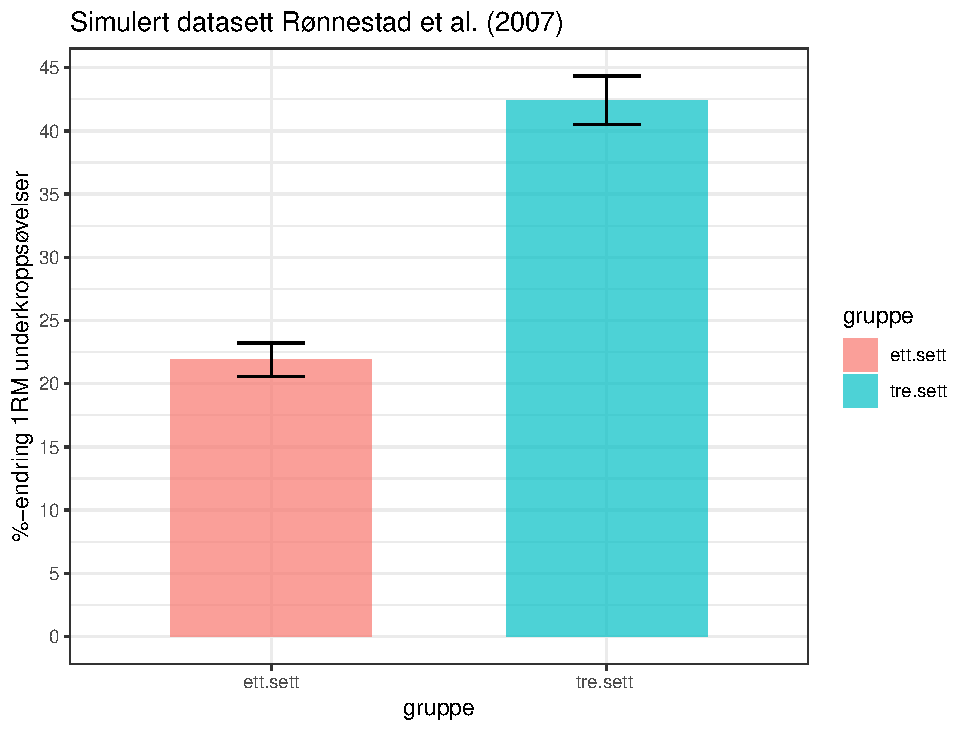
\includegraphics[width=0.8\linewidth]{02-datasett_files/figure-latex/nice-fig-1} 

}

\caption{Here is a nice figure!}\label{fig:nice-fig}
\end{figure}

Et stolpediagram er pent å se på, men er egentlig designet for å kategoriske data. For eksempel er det fint å bruke dette når vi skal presentere frekvensen antall som har kjørt bil til skolen og antall personer som har gått. Les \href{https://journals.plos.org/plosbiology/article?id=10.1371/journal.pbio.1002128}{Beyond Bar and Line Graphs: Time for a New Data Presentation Paradigm}. Deretter svar på følgende spørsmål for å se om du har forstått problemene ved å bruke stolpediagram på kontinuerlig data.

``Stolpediagram er designet for kontinuerlig kategorisk data. Høyden på stolpen representerer (bruk det norske begrepet!), hvilket vil si at det også må ligge noen observasjoner over og under stolpen. Man blir dermed ikke lurt lurt ved å bruke et stolpediagram''. Et stolpediagram viser heller ikke standard error standardavvik CI fordelingen av observasjonene, og dette spesielt være problematisk ved store små. Derfor anbefaler forfatterne i artikkelen at man viser dataen mer ved å for eksempel bruke et bar graph scatterplot. Hvis man likevel ønsker å bruke et stolpediagram for å presentere dataen er det viktig at man forteller om man har brukt SE, SD eller CI. Stanard error for gjennomsnittet regnes ved å ta \(SD/sqrt(N)\), så ved store utvalg vil standard error være høyt lite. Standardavviket er kun \(sqrt(varians/n-1)\), så denne vil i større mindre grad være påvirket av utvalgsstørrelsen".

\hypertarget{koding-av-kategoriske-variabler}{%
\chapter{Koding av kategoriske variabler}\label{koding-av-kategoriske-variabler}}

I tabellen på s. kan du se at vi har en tabell med tre kolonner: en kolonne for hver variabel vi har i vårt datasett. Variabelen \textbf{gruppe} er en kategorisk vaiabel som har to ulike verdier: ``ett.sett'' og ``tre.sett''. Dette er de to gruppene som vi skal teste om er forskjellige. I programmeringsverdenen kalles disse denne typen data for et tekstobjekt, ``strings'' (python/javascript) eller ``characters'' (R). På norsk kalles disse verdiene for ord. Uansett navn er problemet at vi ikke kan putte ord inn i en statistisk modell; vi er nødt til å representere denne kategoriske vaiabelen med tallverdier. Det er flere måter å gjøre dette på, men de forskjellige måtene gir ulik resultat. Derfor må vi vie en god del tid på dette. Vi går gjennom to måter å gjøre dette på.

\hypertarget{dummykoding}{%
\section{Dummykoding}\label{dummykoding}}

En vanlig metode kalles \textbf{dummykoding} eller \textbf{treatment-koding}. Den går ut på å lage en eller flere variabler med 0 og 1 som de to mulige verdiene. Antall variabler vi trenger avhenger av antall grupper vi vil sammenligne. Siden vårt datasett kun inneholder to grupper, så trenger vi kun en variabel. Vi kan den ene gruppen og den andre 1. Hovedregelen er at vi gir 0 til baselinegruppe og 1 til den eksperimentelle gruppen. Vi gir derfor 0 til 1.sett-gruppen og 1 til 3.sett-gruppen. Gjør dette før du går videre.

I R og Jamovi kan du gjøre det med følgende if/else statement. I R kan du bruke følgende kode:

\begin{Shaded}
\begin{Highlighting}[]
\CommentTok{\#lager et nytt objekt som heter dummykodet.dat}
\NormalTok{dummykodet.dat }\OtherTok{\textless{}{-}}\NormalTok{ dat }\SpecialCharTok{\%\textgreater{}\%}
  \CommentTok{\# her lager jeg en ny kolonne som heter dummykoder. If gruppe == \textquotesingle{}ett.sett\textquotesingle{}, gi verdien 0, else gi de 1.}
  \FunctionTok{mutate}\NormalTok{(}\AttributeTok{dummykodet =} \FunctionTok{if\_else}\NormalTok{(gruppe }\SpecialCharTok{==} \StringTok{"ett.sett"}\NormalTok{, }\DecValTok{0}\NormalTok{, }\DecValTok{1}\NormalTok{))}
\end{Highlighting}
\end{Shaded}

I jamovi ville jeg sett følgende video: \url{https://www.youtube.com/watch?v=iITxK27LfZk}

\begin{table}

\caption{\label{tab:unnamed-chunk-4}Dummy koding}
\centering
\begin{tabular}[t]{r|l|r|r}
\hline
individ & gruppe & rm & dummykodet\\
\hline
1 & tre.sett & 40.467 & 1\\
\hline
2 & tre.sett & 49.072 & 1\\
\hline
3 & tre.sett & 47.941 & 1\\
\hline
4 & tre.sett & 44.514 & 1\\
\hline
5 & tre.sett & 52.288 & 1\\
\hline
6 & tre.sett & 40.018 & 1\\
\hline
7 & tre.sett & 49.484 & 1\\
\hline
8 & tre.sett & 29.210 & 1\\
\hline
9 & tre.sett & 40.593 & 1\\
\hline
10 & tre.sett & 37.587 & 1\\
\hline
11 & tre.sett & 35.427 & 1\\
\hline
12 & tre.sett & 42.494 & 1\\
\hline
13 & ett.sett & 17.706 & 0\\
\hline
14 & ett.sett & 17.072 & 0\\
\hline
15 & ett.sett & 18.268 & 0\\
\hline
16 & ett.sett & 25.426 & 0\\
\hline
17 & ett.sett & 32.703 & 0\\
\hline
18 & ett.sett & 19.102 & 0\\
\hline
19 & ett.sett & 22.238 & 0\\
\hline
20 & ett.sett & 22.271 & 0\\
\hline
21 & ett.sett & 26.179 & 0\\
\hline
22 & ett.sett & 20.349 & 0\\
\hline
23 & ett.sett & 23.528 & 0\\
\hline
24 & ett.sett & 17.960 & 0\\
\hline
\end{tabular}
\end{table}

\hypertarget{kontrastkoding}{%
\section{Kontrastkoding}\label{kontrastkoding}}

Kontrastkoding er et alternativ til dummykoding. Det er en regel som er viktig å følge for å ha en gyldig kontrastkode, og det er at summen av kontrastkodene blir 0. For eksempel er -0.5 og 0.5 gyldige kontrastkoder fordi summen av disse blir 0. Det samme er -10 og +10. 0 og 1 derimot, slik vi har med en dummykodet variabel, er ikke er en gyldig kontrastkode fordi summen av disse blir 1. \textbf{Hvilke verdier vi velger å bruke på vår kontrastkodede variabel betyr ingenting for den statistiske test vi gjennomfører, men gjør at vi må fortolke resultatene litt forskjellig}. Med en kontrastkode på +10 og -10 er det en 20 enhets forskjell, mens det ved +0.5 og -0.5 kun er enhet forskjell.

\begin{Shaded}
\begin{Highlighting}[]
\CommentTok{\#lager et nytt objekt som heter dummykodet.dat}
\NormalTok{kontrastkodet.dat }\OtherTok{\textless{}{-}}\NormalTok{ dummykodet.dat }\SpecialCharTok{\%\textgreater{}\%}
  \CommentTok{\# her lager jeg en ny kolonne som heter kontrastkodet. If gruppe == \textquotesingle{}ett.sett\textquotesingle{}, gi verdien {-}0.5, else gi de +0.5}
  \FunctionTok{mutate}\NormalTok{(}\AttributeTok{kontrastkodet =} \FunctionTok{if\_else}\NormalTok{(gruppe }\SpecialCharTok{==} \StringTok{"ett.sett"}\NormalTok{, }\SpecialCharTok{{-}}\FloatTok{0.5}\NormalTok{, }\SpecialCharTok{+}\FloatTok{0.5}\NormalTok{)}
\NormalTok{         )}
\end{Highlighting}
\end{Shaded}

\begin{table}

\caption{\label{tab:unnamed-chunk-6}Kontrastkoding}
\centering
\begin{tabular}[t]{r|l|r|r|r}
\hline
individ & gruppe & rm & dummykodet & kontrastkodet\\
\hline
1 & tre.sett & 40.467 & 1 & 0.5\\
\hline
2 & tre.sett & 49.072 & 1 & 0.5\\
\hline
3 & tre.sett & 47.941 & 1 & 0.5\\
\hline
4 & tre.sett & 44.514 & 1 & 0.5\\
\hline
5 & tre.sett & 52.288 & 1 & 0.5\\
\hline
6 & tre.sett & 40.018 & 1 & 0.5\\
\hline
7 & tre.sett & 49.484 & 1 & 0.5\\
\hline
8 & tre.sett & 29.210 & 1 & 0.5\\
\hline
9 & tre.sett & 40.593 & 1 & 0.5\\
\hline
10 & tre.sett & 37.587 & 1 & 0.5\\
\hline
11 & tre.sett & 35.427 & 1 & 0.5\\
\hline
12 & tre.sett & 42.494 & 1 & 0.5\\
\hline
13 & ett.sett & 17.706 & 0 & -0.5\\
\hline
14 & ett.sett & 17.072 & 0 & -0.5\\
\hline
15 & ett.sett & 18.268 & 0 & -0.5\\
\hline
16 & ett.sett & 25.426 & 0 & -0.5\\
\hline
17 & ett.sett & 32.703 & 0 & -0.5\\
\hline
18 & ett.sett & 19.102 & 0 & -0.5\\
\hline
19 & ett.sett & 22.238 & 0 & -0.5\\
\hline
20 & ett.sett & 22.271 & 0 & -0.5\\
\hline
21 & ett.sett & 26.179 & 0 & -0.5\\
\hline
22 & ett.sett & 20.349 & 0 & -0.5\\
\hline
23 & ett.sett & 23.528 & 0 & -0.5\\
\hline
24 & ett.sett & 17.960 & 0 & -0.5\\
\hline
\end{tabular}
\end{table}

Spørsmålet dere sikkert lurer på er hvorfor vi dummykoder og kontrastkoder gruppe-variabelen vår. Det korte svaret er at vo gjør det fordi vi skal se at disse to måtene å kode på produserer forskjellige svar.

\hypertarget{bygge-statistisk-modeller}{%
\chapter{Bygge statistisk modeller}\label{bygge-statistisk-modeller}}

\hypertarget{om-modellbygging}{%
\section{Om modellbygging}\label{om-modellbygging}}

Modellbygging er en av forskernes kjerneoppgaver. Hovedideen med slik modellbygging er at vi ønsker å bygge en statistisk modell til å predikere hva en person faktisk har hatt som skår på den avhengige variabelen. Til dette kan vi bruke en lineær modell som er en variant av følgende ligning:

\[
data_i = (modell) + error_i
\]

\textbf{Data} er den avhengige variabelen som vi har målt hos alle deltakerne og som vi kan bruke en modell til å predikere. Å predikere er et verb som benyttes mye i statistikken, og er synonymt med å forutsi. Min måte å tenke på det er at vi ønsker å si hva en person hadde som faktisk observasjon på den målte avhengig variabelen. Legg også merke til den lille \emph{i}-en som står bak data og error i ligningen. Denne betyr individ, og sier at vi kan predikere et individ sin skår på den avhengige variabelen med modellen som vi har bygget. \textbf{Modell} er egentlig bare en representasjon av denne dataen, mens \textbf{error} er hvor mye modellen bommer fra den faktisk observasjonen (dvs. data). Dette blir kanskje mer konkret om vi bruker et eksempel:

La oss si at du er lege og at du får inn en pasient som sier hun har feber. Du vet at den normale kroppstemperaturen er 37 så dette blir modellen din.

\[
data = 37 + error
\]
Det neste du gjør er å ta en febermåling av pasienten, og du måler kroppstemperaturen hennes til å være 40.

\[
40 = 37 + error
\]
Modellen din bommer derfor mer 3, fordi 40-37 = 3.

\[
40 = 37 + 3
\]
Formelt sett regner vi error for en hvilken som helst modell ved å få error alene i ligningen.

\[
data = modell + error
\]
\[
error = data - modell
\]
\[
3 = 40 - 37
\]
Dette var en superenkel modell, men viser hvordan vi kan bruke slike modeller. Ofte bygger vi ikke modeller for ett individ, men flere. Tenk bare hvor mange deltakere vi har med i en studie. Modellen vi bygger bør være en god representasjon av alle disse individene. Med andre ord bør erroren være så liten som mulig. \textbf{Dette er essensielt!} Vi ønsker å bygge statistiske modeller som er gode, og vi ønsker å sammenligne ulike modeller for å se hvilke av disse modellene som reduserer erroren mest mulig.

Det er en mer presis og korrekt måte å skrive ligningen over på, og som du ofte ser i artikler og statistikkbøker:

\[
data = (modell) + error
\]
\[
Y_i = (b_0 + b_1X_i) + error
\]
Her er \$ \textbf{Y\_i} \$ den avhengige variabelen som vi faktisk har målt for et individ, \emph{i}. \textbf{X\_i} er dette individets faktiske måling på variabel X, som vi ofte kaller for prediktorvariabel. Som det fremgår av den siste ligningen har også \$ b1 \$ hektet på seg. Denne forteller oss forholdet mellom prediktorvariabelen (Xi) og den avhengig variabelen (). Vi skriver den liten liten \emph{b} fordi dette er noe vi estimerer fra et utvalg. \textbf{b0} er vår prediksjon når Xi er \textbf{null} og \textbf{0}.

I figurene under ser tre ulike modelle med uinteressante X og Y variabler. Alle har samme b0, mens de har forskjellig b1. Husk at b1 forteller om forholdet mellom X og Y. I modell A ser du at når X øker så øker Y med 0.4 for hver enhets økning i X. I modell B er det ingen relasjon mellom X og Y, så for en enhets økning X, vil Y være den samme. I modell C er det en negativ relasjon mellom X og Y. Denne modellen sier at for en enhets økning i X, vil vi forvente Y går ned med 0.4 (siden den er negativ).

\begin{figure}

{\centering 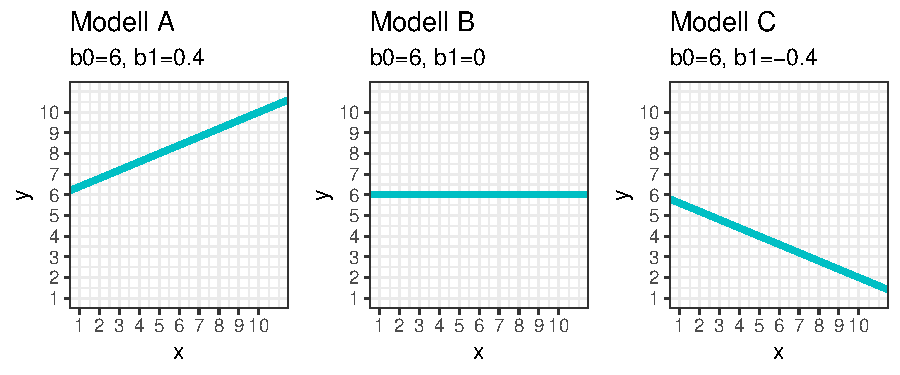
\includegraphics[width=1\linewidth]{04-h0_files/figure-latex/unnamed-chunk-2-1} 

}

\caption{**CAPTION THIS FIGURE!!**}\label{fig:unnamed-chunk-2}
\end{figure}

\hypertarget{test-kunnskapen-din}{%
\subsection{Test kunnskapen din}\label{test-kunnskapen-din}}

La oss si at vi hatt med et målt et individ sin \textbf{X} og \textbf{Y} (du kan bytte ut X og Y med hvilken som helst variabel (f.eks. høyde, vekt), hvis du vil). Individet sitt mål på X er 8. Hvis du bruker modell A, hva vil du forvente at denne personen har på \emph{Y}?

.

I figuren ser du tre modeller som har ulike b1, men samme b0. b0 er verdien på Y når X = null/0.

\begin{figure}

{\centering 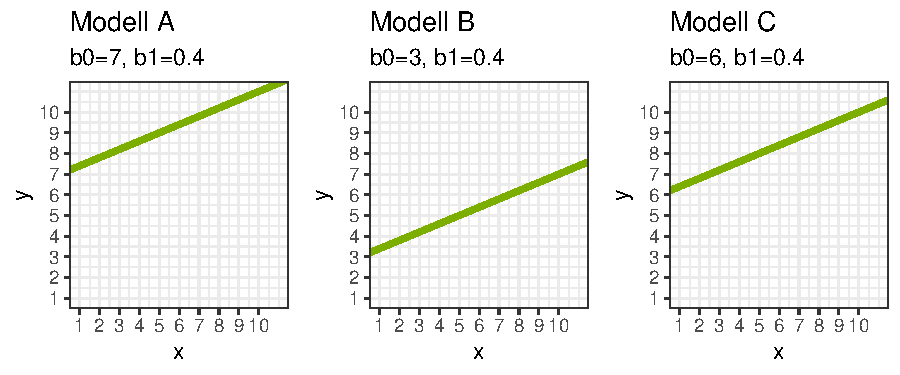
\includegraphics[width=1\linewidth]{04-h0_files/figure-latex/unnamed-chunk-3-1} 

}

\caption{**CAPTION THIS FIGURE!!**}\label{fig:unnamed-chunk-3}
\end{figure}

\hypertarget{test-kunnskapen-din-1}{%
\subsection{Test kunnskapen din}\label{test-kunnskapen-din-1}}

La oss si at vi hatt med et målt et individ sin \textbf{X} og \textbf{Y} (du kan bytte ut X og Y med hvilken som helst variabel (f.eks. høyde, vekt), hvis du vil). Individet sitt mål på X er 3. Hvis du bruker modell B, hva vil du forvente at denne personen har på \emph{Y}?

.

\hypertarget{modellbygging-med-null-hypothesis-significance-testing-nhst}{%
\section{Modellbygging med `Null-Hypothesis Significance Testing (NHST)'}\label{modellbygging-med-null-hypothesis-significance-testing-nhst}}

Nå som du har en fått en innføring i hvordan du kan bygge modeller er det på tide at vi begynner å spesifisere hvilke modeller vi skal bygge. Som du sikkert er kjent med jobber forskere innenfor et paradigme som kalles for \textbf{Null-Hypothesis Significance Testing (NHST)}. Dette går ut på at forskeren fremstiller to hypoteser:

\begin{enumerate}
\def\labelenumi{\arabic{enumi}.}
\tightlist
\item
  \textbf{H0}: En null-hypotese som sier at det ikke er noen effekt (f.eks. ingen forskjeller mellom grupper, ingen sammenheng mellom variablene)
\item
  \textbf{H1}: En alternativ/eksperimentell hypotese som sier at det er en effekt (f.eks. det er en forskjell mellom gruppene)
\end{enumerate}

For å teste disse hypotesene må forskeren bygge to modeller: en modell for null-hypotesen (vi kaller denne for \textbf{null-modellen}) og en \textbf{alternativ-modell}. Vi regner ut hvor mye error det er i hver av disse modellene for å se hvilke av disse modellene det er klokt å benytte. Husk at målet er å benytte modeller som er gode og som har lite error. Hvis null-modellen er god nok, så er det ikke noe poeng å bruke den alternative modellen. Men hvis den alternative modellen er mye bedre enn null-modellen, da bør benytte denne. Forskeren gjennomfører deretter en \textbf{statistisk test} som representerer den alternative hypotesen. Utfallet av testen er en \textbf{verdi}, for eksempel en \emph{z-verdi}, \emph{t-verdi} eller \emph{f-verdi}, som vi kan bruke til å regne ut sannsynligheten for, gitt at null-hypotesen er sann. Forskjellige tester opererer med forskjellige navn på verdiene sine (sorry, men det er bare slik det er).

\begin{figure}

{\centering 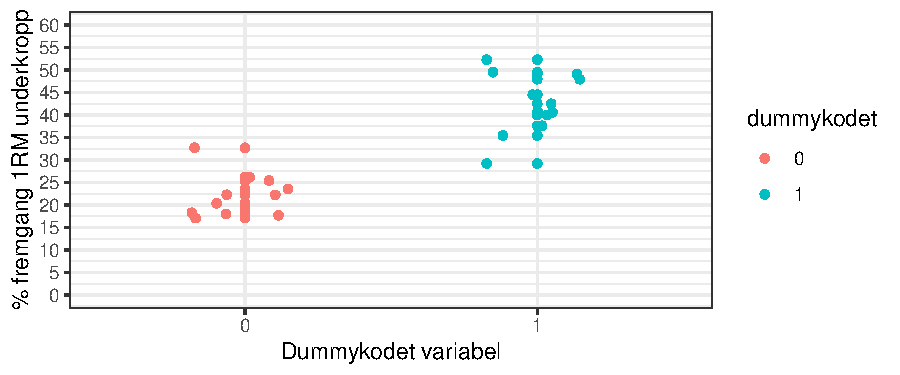
\includegraphics[width=1\linewidth]{04-h0_files/figure-latex/unnamed-chunk-4-1} 

}

\caption{**CAPTION THIS FIGURE!!**}\label{fig:unnamed-chunk-4}
\end{figure}

\hypertarget{null-modellen-null-hypotesen}{%
\section{Null-modellen (null-hypotesen)}\label{null-modellen-null-hypotesen}}

I vår studie ønsker vi å teste om det er forskjeller mellom de to gruppene som har blitt disponert for ulikt treningsopplegg (3 versus 1 sett). Husk at vi har laget en variabel hvor vi har kodet disse som 0 og 1. Null-hypotesen er at det ikke er noen forskjeller mellom gruppene. En annen måte å formulere dette på er om vi blir bedre til å predikere et individs skår hvis vi vet hvilken gruppe de tilhører eller om vi kun trenger en enkel modell. Den enkleste modellen vi kan benytte er gjennomsnittet i \% fremgang 1RM for alle deltakerne. Dette er modellen som representerer null-hypotesen. Med andre ord vår null-modell

\[
Y_i = (b_0) + error
\]
\[
fremgang.1RM = (mean) + error
\]
Det er ofte enklere å se denne modellen i tabellform, slik som dere ser under.

\label{tab:unnamed-chunk-6}Null-modellen (mean)

individ

gruppe

rm

modell.mean

error

1

tre.sett

40.467

32.162

8.305

2

tre.sett

49.072

32.162

16.910

3

tre.sett

47.941

32.162

15.779

4

tre.sett

44.514

32.162

12.352

5

tre.sett

52.288

32.162

20.125

6

tre.sett

40.018

32.162

7.855

7

tre.sett

49.484

32.162

17.322

8

tre.sett

29.210

32.162

-2.952

9

tre.sett

40.593

32.162

8.431

10

tre.sett

37.587

32.162

5.424

11

tre.sett

35.427

32.162

3.264

12

tre.sett

42.494

32.162

10.331

13

ett.sett

17.706

32.162

-14.457

14

ett.sett

17.072

32.162

-15.091

15

ett.sett

18.268

32.162

-13.894

16

ett.sett

25.426

32.162

-6.736

17

ett.sett

32.703

32.162

0.541

18

ett.sett

19.102

32.162

-13.060

19

ett.sett

22.238

32.162

-9.924

20

ett.sett

22.271

32.162

-9.891

21

ett.sett

26.179

32.162

-5.983

22

ett.sett

20.349

32.162

-11.814

23

ett.sett

23.528

32.162

-8.635

24

ett.sett

17.960

32.162

-14.203

La oss prøve hvordan denne modellen virker. For individ 1 målte vi en fremgang i 1RM underkropp på \textbf{40.467}, men modellen vår sa \textbf{32.162}. Så modellen bommet med 8.305, dvs. en error på \textbf{8.305}.
\[
fremgang.1RM = (mean) + error
\]
\[
40.467 = 32.162 + 8.305
\]
Prøv modellen du også: For individ nr. 8, sier modellen at individet hadde en skår på , men denne personen hadde faktisk en skår på . Modellen bommet derfor med .

Vi kan fortsette slik for alle deltakerne vi har hatt med i studien. Husk at vi ikke er interessert i hvir mye bommer for hvert enkelt individ, men for alle indivene. Summer derfor all erroren for alle indidene, hvilket tall får du da? null 0 3 -3. (tenk over hvorfor du får dette svaret før du leser videre)

Som du så i forrige oppgave blir det feil å summere alle erroren, men ved å regne \textbf{Sum of Squared Error} løser vi dette problemet effektivt. Det vi gjør er å gange error med seg selv (error\^{}2) før vi summerer alt dette sammen.

Hvis vi regner ut \textbf{Sum of Squared Error} for null-modellen fpr vi: . Dette tallet er viktig! Dette er null-hypotesen vår. Hvis det ikke er noen forskjell mellom de to treningsgruppene våre er det like greit å bruke denne null-modellen. Men hvis vi finner ut at modellen vår blir bedre (dvs. reduserer Sum of Squared Error) ved å legge til en prediktorvariabel som består er av gruppevariabelen vår, da bør vi gjøre dette.

Før du går videre er det greit å visualisere hvordan null-hypotesen ser ut rent visuelt. Den prikkete streken i figuren under representerer modellen vår som er mean. Som du ser, så gjør den ingen justeringer for de ulike individene. Erroren er avstanden fra den linjen og opp til hvert datapunkt.

\begin{figure}

{\centering 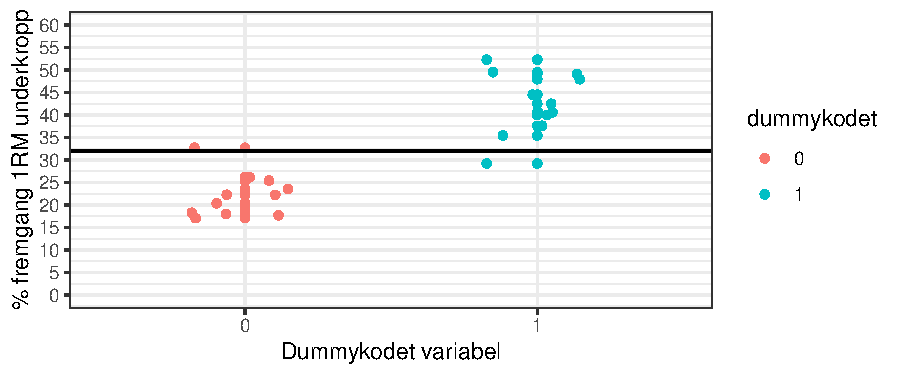
\includegraphics[width=1\linewidth]{04-h0_files/figure-latex/unnamed-chunk-8-1} 

}

\caption{**CAPTION THIS FIGURE!!**}\label{fig:unnamed-chunk-8}
\end{figure}

\hypertarget{h1-alternativ-modell-alternativ-hypotese}{%
\section{H1: Alternativ modell (alternativ hypotese)}\label{h1-alternativ-modell-alternativ-hypotese}}

I forrige avsnitt sa vi at \textbf{null-hypotesen (H0)} reresenterer en en modell som gir samme prediksjon for alle deltakerne som var med i studien uavhengig av hvilken treningsgruppe de tilhører. Vi kalte denne for null-modellen. Vi regnet oss også frem til at denne modellen ga oss en Som of Squared error på 3243.784.

\[
Y_i = (b_0) + error_i
\]
\[
Fremgang.1RM_i = (mean) + error_i
\]

Spørsmålet vi skal stille i dette avsnittet er om vi kan redusere error fra denne ved å benytte en mer kompleks modell som benytter (vår dummykodede kategoriske variabel) som prediktorvariabel:
\[
Y_i = (b_0 + b_1X_i) + error
\]
Prediktorvariabelen b1 er en gruppevariabelen vår som vi dummykodet med tallene 0 og 1.

\[
Fremgang.1RM_i = b_0 + b_1(Gruppe) + error_i
\]
For å fokusere på holde dette på et overordnet nivå, så vil jeg gi dere de estimerte verdiene for b0 og b1. Målet er å vise dere hvordan denne modellen fungerer. Senere skal gå gjennom hvordan vi regner ut disse verdiene.

\[
Fremgang.1RM_i = b_0(21.90) + b_1(20.52*Gruppe) + error_i
\]
Modellen sier at vi har en intercept på 21.90. Dette er forventede verdien på Y (Fremgang.1RM) når prediktorvariabelen er 0. Modellen sier også at b1 er 20.52. Med andre ord den forventede økning i Y for en enhets økning i X. Husk at vi lagde en gruppe-variabel der vi kodet de to gruppene våre med 0 og 1. Så hvis et individ tilhørte gruppe 0, blir vår prediksjon:

\[
Fremgang.1RM_i = 21.90 + b_1(20.52*0) + error_i
\]
0*20.52 = 0, så blir stående igjen med b0, vår prediksjon av Y når er nulll
\[
Fremgang.1RM_i = 21.90 + 0 + error_i
\]
\[
Fremgang.1RM_i = 21.90 + error_i
\]
Hvis individet derimot tilhører 1 predikerer modellen at individet sin skår blir 42.48.

\[
Fremgang.1RM_i = 21.90 + b1(20.52*1) + error_i
\]
\[
Fremgang.1RM_i = 42.48 + error_i
\]
Visualisert fremstilt blir modellen vår seendes slik ut:

\begin{Shaded}
\begin{Highlighting}[]
\FunctionTok{ggplot}\NormalTok{(dat, }\FunctionTok{aes}\NormalTok{(dummykodet, rm, }\AttributeTok{color=}\NormalTok{dummykodet)) }\SpecialCharTok{+}
  \FunctionTok{geom\_point}\NormalTok{()}\SpecialCharTok{+}
  \FunctionTok{scale\_y\_continuous}\NormalTok{(}\AttributeTok{breaks =} \FunctionTok{seq}\NormalTok{(}\DecValTok{0}\NormalTok{, }\DecValTok{60}\NormalTok{, }\DecValTok{5}\NormalTok{)) }\SpecialCharTok{+}
  \FunctionTok{coord\_cartesian}\NormalTok{(}\AttributeTok{ylim =} \FunctionTok{c}\NormalTok{(}\DecValTok{0}\NormalTok{, }\DecValTok{60}\NormalTok{)) }\SpecialCharTok{+}
  \FunctionTok{geom\_jitter}\NormalTok{(}\AttributeTok{width =} \FloatTok{0.2}\NormalTok{) }\SpecialCharTok{+} 
  \FunctionTok{stat\_summary}\NormalTok{(}\AttributeTok{geom =} \StringTok{"line"}\NormalTok{, }\AttributeTok{fun =}\NormalTok{ mean, }\AttributeTok{group =} \DecValTok{1}\NormalTok{, }\AttributeTok{color=}\StringTok{"black"}\NormalTok{, }\AttributeTok{linetype=}\StringTok{"dotted"}\NormalTok{, }\AttributeTok{size=}\FloatTok{1.2}\NormalTok{) }\SpecialCharTok{+}
  \FunctionTok{labs}\NormalTok{(}\AttributeTok{y=}\StringTok{"\% fremgang 1RM underkropp"}\NormalTok{, }\AttributeTok{x=}\StringTok{"Dummykodet variabel"}\NormalTok{) }\SpecialCharTok{+}
  \FunctionTok{theme\_bw}\NormalTok{()}
\end{Highlighting}
\end{Shaded}

\begin{figure}

{\centering 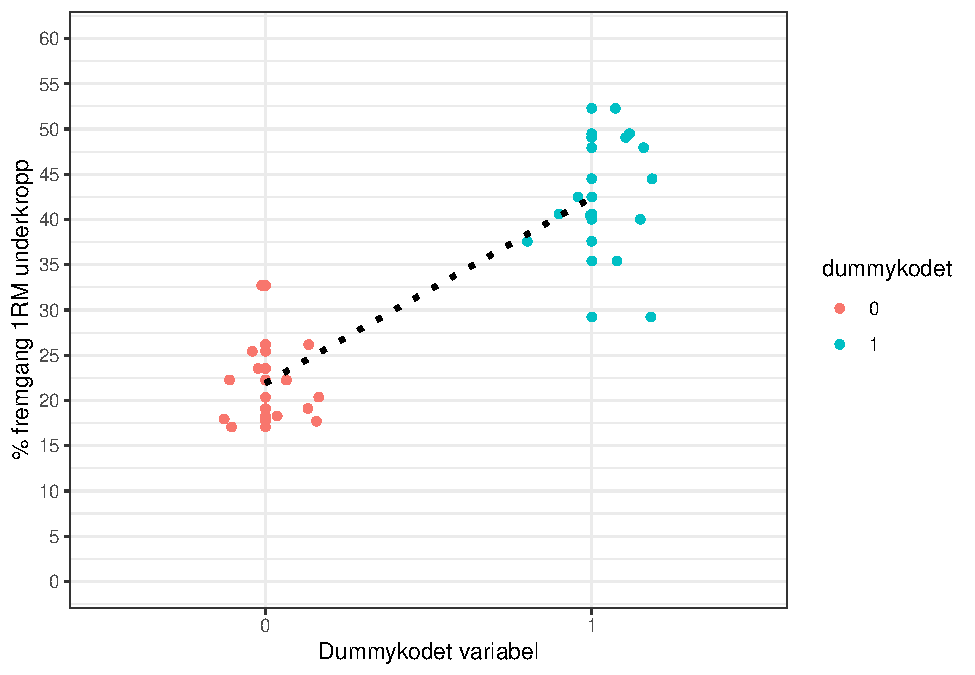
\includegraphics[width=1\linewidth]{04-h0_files/figure-latex/unnamed-chunk-9-1} 

}

\caption{**CAPTION THIS FIGURE!!**}\label{fig:unnamed-chunk-9}
\end{figure}

\textbf{Oppgaver}
Tabellen under viser 6 individer som tilhørte treningsgruppe. Du ser deres faktiske fremgang i 1RM kolonnen. La oss bruke det vi har lært til å predikere disse personene sin fremgang. Vi bruker samme modell som over

\[
Fremgang.1RM_i = b_0(21.90) + b_1(20.52*Gruppe) + error_i
\]
a) Hva predikerer modellen at individ nummer 3 hadde i skår? (to desimaler)

\begin{enumerate}
\def\labelenumi{\alph{enumi})}
\setcounter{enumi}{1}
\tightlist
\item
  Hva hadde individ nr i skår?
\end{enumerate}

\begin{enumerate}
\def\labelenumi{\alph{enumi})}
\setcounter{enumi}{2}
\tightlist
\item
  hvor mye error blir det?
\end{enumerate}

\begin{enumerate}
\def\labelenumi{\alph{enumi})}
\setcounter{enumi}{3}
\tightlist
\item
  i Squared Error blir denne erroren?
\end{enumerate}

\begin{enumerate}
\def\labelenumi{\alph{enumi})}
\setcounter{enumi}{4}
\tightlist
\item
  nå som du har jobbet med denne modellen, så lurer jeg på om det er noe kjent med disse verdiene i modellen. Gå tilbake til {[}link{]} hvis du trenger et hint.
\end{enumerate}

bo er (norskt ord) for gruppen som er kodet med 0. b1 er (norsk ord) mellom gruppen som er kodet med 0 og gruppen som er kodet med 1. b0 + b1 (norsk ord) for gruppen som er kodet med 1.

\begin{table}

\caption{\label{tab:unnamed-chunk-11}Dummy koding}
\centering
\begin{tabular}[t]{r|l|r|r}
\hline
individ & gruppe & rm & dummykodet\\
\hline
1 & tre.sett & 40.467 & 1\\
\hline
2 & tre.sett & 49.072 & 1\\
\hline
3 & tre.sett & 47.941 & 1\\
\hline
4 & tre.sett & 44.514 & 1\\
\hline
5 & tre.sett & 52.288 & 1\\
\hline
6 & tre.sett & 40.018 & 1\\
\hline
\end{tabular}
\end{table}

I forrige oppgave regnet du ut error for ett enkelt individ. Men vi er interessert i den totale erroren for modellen. Formelen for denne er:

total error in den alternative modellen:

SS\_R = \(\sum_{n=1}^N (observert_i - modell_i)^2\)

Med andre ord er det kvadraten av den faktiske observasjonen - hva modellen sa. Bruk formelen til å regne ut dette. (to desimaler

\hypertarget{variansanalyse-anova-tabell}{%
\section{Variansanalyse (ANOVA-tabell)}\label{variansanalyse-anova-tabell}}

Nå som vi har regnet ut hvor mye error det er i hver av disse modellene - null-modellen og den alternative modellen - er det klart for å gjøre en sammenligning av disse modellene. Modellene vi sammenligner er om alternative-modellen reduserer error mer enn null-modellen. Fra figurene under kan det slik ut; linjen til høyre ser ut til å ligge nærmere observasjonene enn linjen i figuren til venstre.

\begin{figure}

{\centering 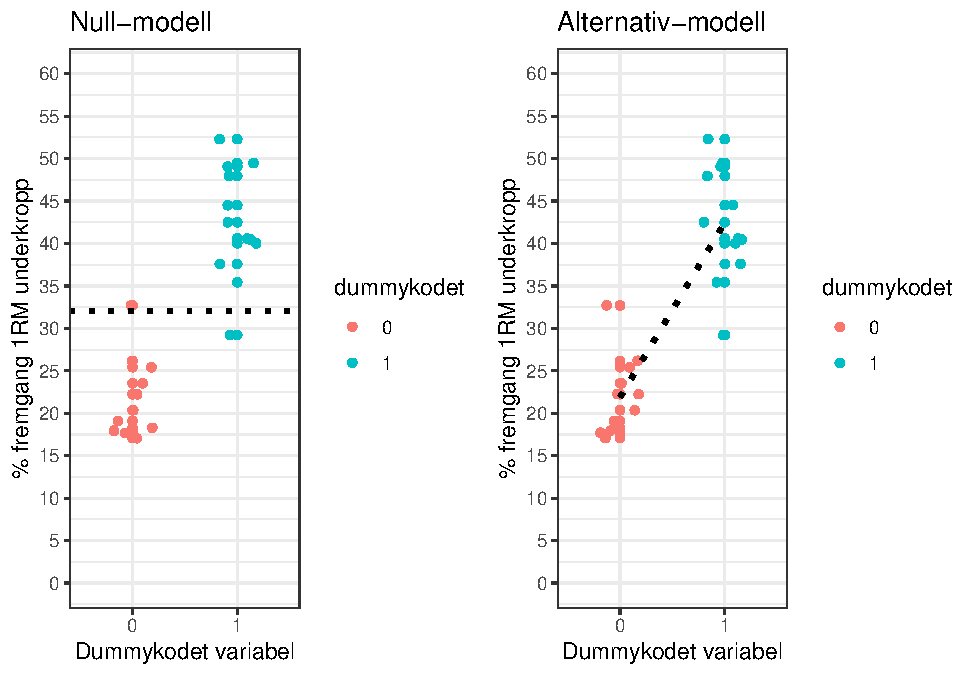
\includegraphics[width=1\linewidth]{04-h0_files/figure-latex/unnamed-chunk-12-1} 

}

\caption{**CAPTION THIS FIGURE!!**}\label{fig:unnamed-chunk-12}
\end{figure}

\textbf{The total sum of squares (SST)} = \textbf{3243.784}
(SST) er hvor mye error vi får ved å bruke null-modellen.

\textbf{The residual sum of squares (SSR)} = \textbf{716.3}
(dette er hvor mye error som er igjen etter at vi brukte modellen vår)

En naturlig ting å gjøre er å regne hvor mye error den alternative modellen vår har redusert error med. Man kaller denne for \textbf{The model sum of squares (SSM)}:

\textbf{The model sum of squares (SSM)} = \textbf{(SST)} - \textbf{(SSR)} =

Hvis vi regner hvor mye error modellen vår har redusert error med, så kan vi se at modellen vår har redusert error med 78 \%. Dette er ekstremt mye, og det er sjeldent man finner en så høy prosent. Denne verdien har mange forskjellige navn i statistikken, *proportional reduction in error (PRE)``, R2 og n2''. Og den er viktig. Jeg velger å bruke R2.

\[
R2 = (SS_T - SS_R) / SS_T
\]
\[
R2 = (3243.784 - 716.3) / 3243.784 
\]

\[
R2 = 0.7791826
\]
Når dere bygger statistiske modeller i R,Jamovi eller SPSS vil dere få en ANOVA-tabell de. Her ser du de samme verdiene som vi har regnet manuelt.

\begin{Shaded}
\begin{Highlighting}[]
\CommentTok{\#aov er en forkortolse for analysis of variance (ANOVA)}
\CommentTok{\#dette er funksjon som kommer mer R.}
\FunctionTok{aov}\NormalTok{(rm }\SpecialCharTok{\textasciitilde{}}\NormalTok{ dummykodet, dat)}
\end{Highlighting}
\end{Shaded}

\begin{verbatim}
## Call:
##    aov(formula = rm ~ dummykodet, data = dat)
## 
## Terms:
##                 dummykodet Residuals
## Sum of Squares   2527.4962  716.2875
## Deg. of Freedom          1        22
## 
## Residual standard error: 5.706008
## Estimated effects may be unbalanced
\end{verbatim}

\hypertarget{f-test}{%
\section{F-test}\label{f-test}}

\begin{verbatim}
## # A tibble: 24 x 6
##       ss sum.ss mod.m  error sum.error   pre
##    <dbl>  <dbl> <dbl>  <dbl>     <dbl> <dbl>
##  1  8.30  3244.  42.4   3.81      716. 0.779
##  2 16.9   3244.  42.4  44.3       716. 0.779
##  3 15.8   3244.  42.4  30.5       716. 0.779
##  4 12.4   3244.  42.4   4.38      716. 0.779
##  5 20.1   3244.  42.4  97.4       716. 0.779
##  6  7.86  3244.  42.4   5.77      716. 0.779
##  7 17.3   3244.  42.4  49.9       716. 0.779
##  8 -2.95  3244.  42.4 174.        716. 0.779
##  9  8.43  3244.  42.4   3.34      716. 0.779
## 10  5.42  3244.  42.4  23.4       716. 0.779
## # ... with 14 more rows
\end{verbatim}

  \bibliography{book.bib,packages.bib}

\end{document}
